\subsection{Overview of exclusivity or diffraction}
\par $pp$ collisions can be grouped into two categories: {\it elastic} and {\it inelastic}. 
During elastic collisions the two protons scatter and emerge out of the collision intact. 
During inelastic collisions either one or both protons may dissociate after collision. Remnants of 
dissociation eventually fragment and hadronize, as discussed in detail in Section~\ref{sec:evgen}. 

\par Diffraction is a term widely used in optical experiments, where a beam of light is separated into 
its multiple components by frequency or wavelength. It is important to note that in that usage the sum of 
the components is exactly the same as the original beam of light. In $pp$ collisions, the term diffraction is 
used to refer to cases where no quantum numbers from the two protons are exchanged during the collision, 
such that the outgoing particles are just components of the incoming protons. 
More precisely, a virtual particle is exchanged during the $pp$ collision.
%, and vacuum quantum numbers are exchanged. 
Elastic processes are trivially diffractive. Inelastic processes 
may or may not be diffractive.

\par Although the $pp$ collision may be at high energy, the actual momentum exchanged during the scattering 
in diffractive processes is by comparison small. In that sense, diffractive processes fall in the `soft' 
energy regime where pertubative QCD does not apply. The Regge Theory~\cite{Costa:2012cb} was the first attempt 
at modelling this phenomenon.\footnote{It is important to note that this theory has since been replaced by QCD.}
Here, the amplitude of the diffractive scattering is given by the sum of all possible virtual exchange particles. 
The most dominant of these virtual particles in this theory is known as the {\it Pomeron}. Several models have 
since substituted this pomeron with other options. One such model is discussed in Section~\ref{sec:exclH}.

\par Inelastic diffractive processes in which one of the protons dissociates is known as Single Dissociation (SD). 
Inelastic diffractive processes in which both protons dissociate is known as Double Dissociation (DD). In this text, 
elastic, SD and DD processes are collectively referred to as {\it exclusive}. The motivation behind this 
nomenclature will become clear in Section~\ref{sec:exclH}. 

\par During an exclusive $pp$ collision photons may be exchanged. This exchange does not change 
the original quantum numbers of the colliding protons. With large enough momentum, the photons may 
interact to form a pair of \Wpm\ ($pp(\gamma\gamma)\to ppWW)$) bosons through one of the vertices shown in Figure~\ref{fig:intGauge}. 
Such a quartic gauge coupling is interesting. Efforts have been made to measure its cross section. 
This process may be elastic, SD or DD. Figure~\ref{fig:exclWW} illustrates these possibilities, where 
$X$ represents the remnants of proton dissociation.      

\begin{figure}[!h]
\begin{subfigure}{0.33\textwidth}
   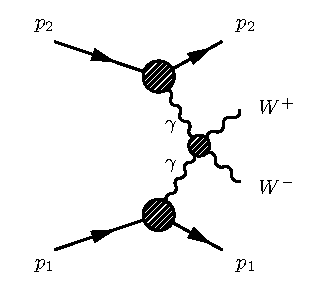
\includegraphics[width=\textwidth]{figures/exclWW.pdf}
\caption{Elastic}
\end{subfigure} % 
\begin{subfigure}{0.33\textwidth}
   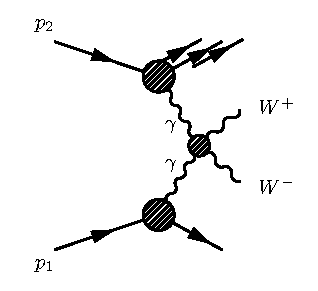
\includegraphics[width=\textwidth]{figures/exclWWsd.pdf}
\caption{Single Dissociative (SD)}
\end{subfigure}%
\begin{subfigure}{0.33\textwidth}
   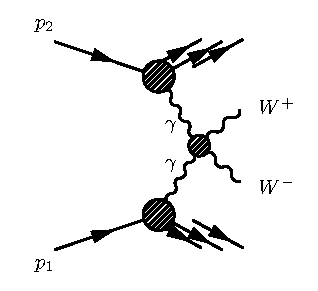
\includegraphics[width=\textwidth]{figures/exclWWdd.pdf}
\caption{Double Dissociative (DD)}
\end{subfigure} % 
\caption{Diagrams showing exclusive processes through photon exchanges, producing a pair of \Wpm\ bosons}
\label{fig:exclWW}
\end{figure}

\par The cross section for the $pp(\gamma\gamma)\to ppWW$ process shown in Figure~\ref{fig:exclWW} is calculated using the 
equivalent photon approximation (EPA)~\cite{EPA0,EPA}. In EPA the photons are described by equivalent photon 
distributions $f(x)$. $f(x)$ is the probability of a photon that carries a fraction of proton energy $x$ to 
be emitted by the proton during the $pp$ collision. The cross section $\sigma_{pp(\gamma\gamma)\to ppWW}^{\text{EPA}}$ is 
then 

\begin{equation}
\sigma_{pp(\gamma\gamma)\to ppWW}^{\text{EPA}} = \iint f(x_1) f(x_2) \sigma_{\gamma\gamma\to WW} (m_{\gamma\gamma}^2) dx_1 dx_2 
\end{equation} 

where $m_{\gamma\gamma}$ is the center of mass energy of the two-photon system. This formulation has been used in several 
experiments to describe exclusive dilepton\footnote{Replace the \Wpm-pair with leptons in Figure~\ref{fig:exclWW}.} 
results~\cite{CDFgg,STARgg,CMSmumu,CMSee}.    
